\documentclass[12pt]{article}

\usepackage{sbc-template}
\usepackage{graphicx,url}
\usepackage[utf8]{inputenc}
\usepackage[brazil]{babel}
\usepackage{subcaption}

     
\sloppy

\title{Análise de Escalabilidade Horizontal em um Cluster Hbase}

\author{Bruno Santos de Lima, Cedryk Augusto dos Santos, Ronaldo Celso Messias Correia }


\address{Faculdade de Ciências e Tecnologia -- Universidade Estadual Paulista (UNESP)\\
  Presidente Prudente -- SP -- Brazil
  \email{bruno.s.lima@unesp.br,cedrykaugusto@gmail.com,ronaldo.correia@unesp.br}
}

\begin{document} 

\maketitle

%Resumo maximo 10 linhas.
%Se o artigo estiver em português o abstract deve estar localizado antes do resumo.

\begin{abstract}
  This meta-paper describes the style to be used in articles and short papers
  for SBC conferences. For papers in English, you should add just an abstract
  while for the papers in Portuguese, we also ask for an abstract in
  Portuguese (``resumo''). In both cases, abstracts should not have more than
  10 lines and must be in the first page of the paper.
\end{abstract}
     
\begin{resumo} 
Com o surgimento do Big Data, identificou-se cenários onde a complexidade lógica existente na modelagem relacional não é necessária e novas soluções com características diferentes foram propostas, denominadas bancos de dados NoSQL. Os bancos de dados NoSQL tem como principal característica o escalonamento horizontal, em que os recursos de um sistema computacional aumenta com a adição de novos nós em um ambiente distribuído (cluster), em vez de substituição por um hardware mais potente. Diante disso, este trabalho avalia o potencial do escalonamento horizontal de um cluster executando o banco de dados NoSQL Hbase, realizando um benchmarking sobre diversos cenários, analisando se com o uso deste paradigma as aplicações podem continuar eficientes e disponíveis independente do tamanho da demanda de armazenamento e de consultas, quando há a adição novos nós no sistema. Os experimentos mostraram que a escalabilidade horizontal existe e é mais evidente, exceto para operações scan (busca), em conjuntos de dados maiores que no contexto dessa pesquisa foram de que neste trabalho foram 100.000 e 1.000.000 de registros de 1KB de tamanho cada e ao se aumentar o número de nós de 1 para 2 e, de 2 para 3 nós. No caso dos testes que executaram operações de busca, não há melhora no desempenho a medida que nós são adicionados ao sistema, devido ao método de busca implementado pelo Hbase ser linear
\end{resumo}


\section{Introdução}
\label{sec:introducao}

Um dos grandes desafios computacionais é o armazenamento e a recuperação de dados
de forma eficiente, para que possam ser acessados rapidamente e que estejam sempre disponíveis a quem os requisite. Durante muitos anos, a solução para a maioria dos problemas dessa área foram os sistemas gerenciadores de banco de dados relacionais (SGBDR), que garantem as propriedades de atomicidade, de consistência, de isolamento e de durabilidade (ACID). Porém, a maioria dos SGBDR’s não atendem mais de forma satisfatória às necessidades de certos cenários identificados com surgimento do Big Data [Brito 2010].

O conceito de Big Data refere-se ao grande volume de dados gerados em diversos domínios de aplicação, como: a Web, dispositivos móveis, sensores, motores de busca e principalmente nas redes sociais; volume este que está na ordem de 1 Zettabyte/dia [Index 2017] e, as tecnologias criadas para a manipulação desses dados garantindo escalabilidade, confiabilidade e tolerância a falhas [Han et al. 2011]. A partir deste conceito, identificou-se que a tecnologia relacional possui grande fragilidade no tratamento de dados classificados como semiestruturados e não estruturados (vídeos, áudios e posts em redes sociais), por exemplo, a dificuldade em acomodá-los no modelo relacional e a dificuldade de implementação distribuída (escalabilidade horizontal) de modo a continuar atendendo às propriedades ACID. A complexidade lógica existente na modelagem relacional somada ao volume exagerado de dados mostrou-se um problema pois pode propiciar deadlocks, problemas de concorrência e lentidão na leitura e escrita dos dados [Han et al. 2011] [Brito 2010].

Como alternativa para esses cenários, surgiram os bancos de dados denominados
NoSQL. Esse termo refere-se aos bancos de dados que não utilizam linguagem SQL para consulta de dados (Not Only SQL), não utilizam do modelo relacional e que em maioria são distribuídos. Tal tecnologia trabalha de forma mais eficiente com grande volume de dados, possibilitando escalar horizontalmente operações por diversos servidores, replicar e distribuir esses dados, adicionar dinamicamente novos atributos aos registros, entre outras. Embora o conceito das ferramentas não relacionais tenha sido apresentado com caráter comparativo, o objetivo destas não é substituir o modelo relacional em todas as situações, apenas nos casos em que é possível adotar uma maior flexibilidade de estruturação e assim, escalonar horizontalmente o sistema de forma eficiente [Brito 2010].

No contexto dente trabalho, foi utilizado o ambiente de desenvolvimento estabelecido pelo framework open-source Hadoop, desenvolvido pela Fundação Apache, que reúne várias ferramentas de manipulação Big Data em um ponto central, envolvendo bancos de dados NoSQL (Hbase), um sistema de arquivos distribuídos denominado Hadoop Distributed File System (HDFS) e um modelo de programação para suportar computações paralelas em grandes coleções de dados em clusters de computadores chamado MapReduce [Apache Hadoop 2016].

O banco de dados Hbase, utilizado neste trabalho, permite o processamento distribuído por meio de clusters. Funciona sobre o HDFS, proporcionando à ferramenta capacidades parecidas ao BigTable /citechang2008bigtable e alta tolerância a falhas ao armazenar grandes quantidades de dados esparsos [Hadoop Hbase 2016].

O objetivo deste trabalho é verificar o potencial desse novo paradigma de armazenamento e recuperação de dados que utiliza de computação distribuída para criar um cenário onde aplicações e serviços continuem eficientes e disponíveis independente do tamanho da demanda de armazenamento e de consultas, apenas pela adição de novos nós ao ambiente distribuído. Dessa forma, foi avaliada a escalabilidade horizontal do banco de dados Hbase por meio de benchmarking com operações read, write, scan e read modifywrite, utilizando o framework Yahoo! Cloud Serving Benchmark (YCSB) a medida em que novos nós são adicionados ao sistema e o tamanho do conjunto de dados é aumentado.

Este trabalho está organizado como segue: A Seção 2 apresenta a fundamentação teórica necessária para a compreensão do trabalho; Na Seção 3 são citados os principais trabalhos relacionados encontrados ao proceder a revisão bibliográfica; A Seção 4 apresenta os cenários de testes utilizados; A Seção 5 exibe a análise quanto aos resultados obtidos e a Seção 6 apresenta as conclusões obtidas.

\section{Background}
\label{sec:background}

\section{Trabalhos Relacionados} 
\label{section:relacionados}

The first page must display the paper title, the name and address of the
authors, the abstract in English and ``resumo'' in Portuguese (``resumos'' are
required only for papers written in Portuguese). The title must be centered
over the whole page, in 16 point boldface font and with 12 points of space
before itself. Author names must be centered in 12 point font, bold, all of
them disposed in the same line, separated by commas and with 12 points of
space after the title. Addresses must be centered in 12 point font, also with
12 points of space after the authors' names. E-mail addresses should be
written using font Courier New, 10 point nominal size, with 6 points of space
before and 6 points of space after.

The abstract and ``resumo'' (if is the case) must be in 12 point Times font,
indented 0.8cm on both sides. The word \textbf{Abstract} and \textbf{Resumo},
should be written in boldface and must precede the text.

\section{Metodologia}
\label{sec:metodologia}

\section{Resultados e Discussões}
\label{sec:resultados}

\begin{figure*}
    \centering
    \begin{subfigure}[b]{0.49\textwidth}
        \centering
        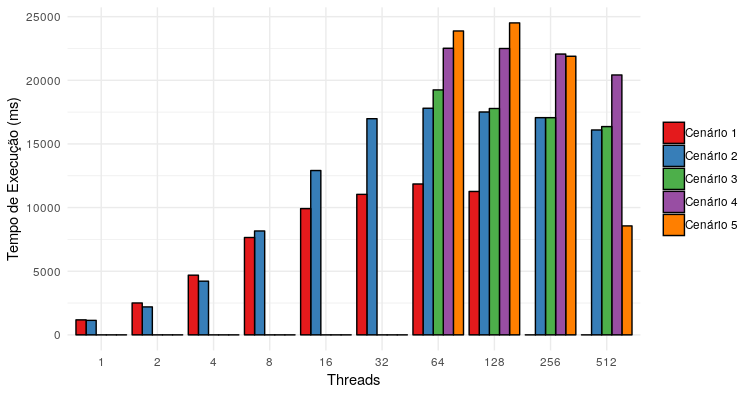
\includegraphics[width=\textwidth]{images/figura11}
        \caption{}
        \label{fig:mean and std of net14}
    \end{subfigure}
        \hfill
    \begin{subfigure}[b]{0.49\textwidth}  
        \centering 
        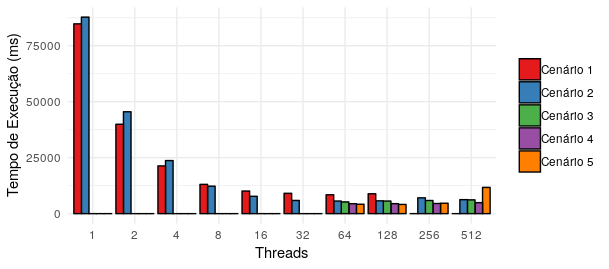
\includegraphics[width=\textwidth]{images/figura12}
        \caption{}%
    \end{subfigure}
    \vskip\baselineskip
    \begin{subfigure}[b]{0.49\textwidth}   
        \centering 
        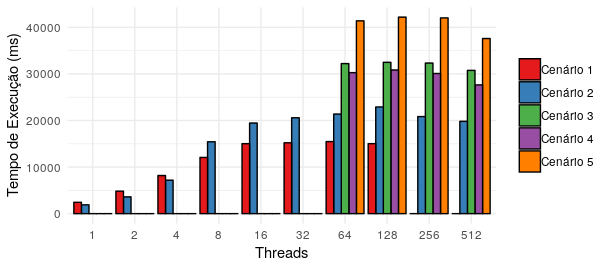
\includegraphics[width=\textwidth]{images/figura13}
        \caption{}
    \end{subfigure}
    \begin{subfigure}[b]{0.49\textwidth}   
        \centering 
        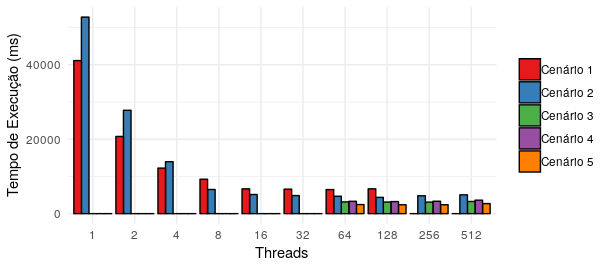
\includegraphics[width=\textwidth]{images/figura14}
        \caption{}
    \end{subfigure}
    \caption{teste}
\end{figure*}


\begin{figure*}
    \centering
    \begin{subfigure}[b]{0.49\textwidth}
        \centering
        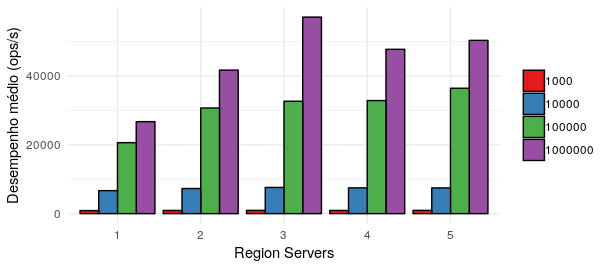
\includegraphics[width=\textwidth]{images/figura15}
        \caption{}
        \label{fig:mean and std of net14}
    \end{subfigure}
        \hfill
    \begin{subfigure}[b]{0.49\textwidth}  
        \centering 
        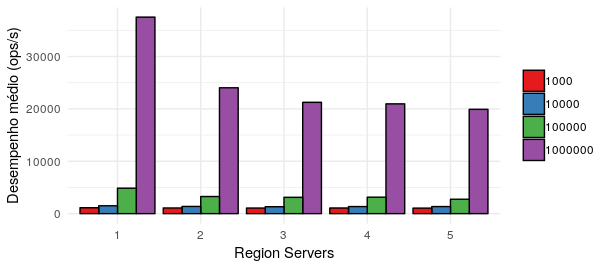
\includegraphics[width=\textwidth]{images/figura16}
        \caption{}%
    \end{subfigure}
    \caption{teste}
\end{figure*}

\begin{figure*}
    \centering
    \begin{subfigure}[b]{0.49\textwidth}
        \centering
        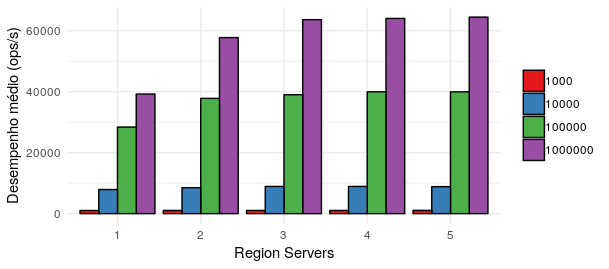
\includegraphics[width=\textwidth]{images/figura17}
        \caption{}
        \label{fig:mean and std of net14}
    \end{subfigure}
        \hfill
    \begin{subfigure}[b]{0.49\textwidth}  
        \centering 
        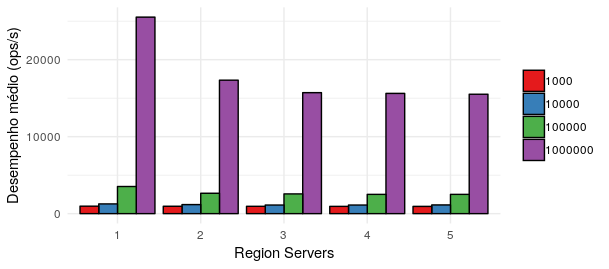
\includegraphics[width=\textwidth]{images/figura18}
        \caption{}%
    \end{subfigure}
    \caption{teste}
\end{figure*}

\begin{figure*}
    \centering
    \begin{subfigure}[b]{0.49\textwidth}
        \centering
        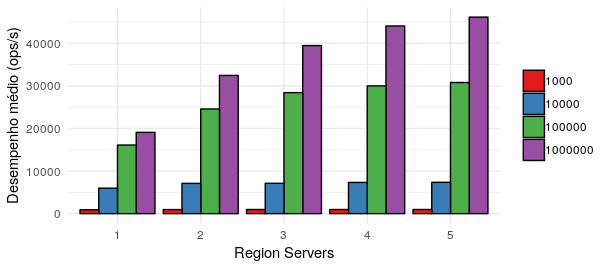
\includegraphics[width=\textwidth]{images/figura19}
        \caption{}
        \label{fig:mean and std of net14}
    \end{subfigure}
        \hfill
    \begin{subfigure}[b]{0.49\textwidth}  
        \centering 
        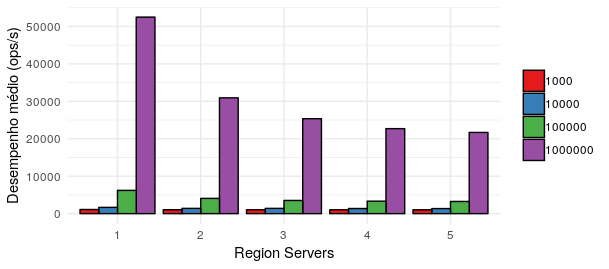
\includegraphics[width=\textwidth]{images/figura20}
        \caption{}%
    \end{subfigure}
    \vskip\baselineskip
    \begin{subfigure}[b]{0.49\textwidth}   
        \centering 
        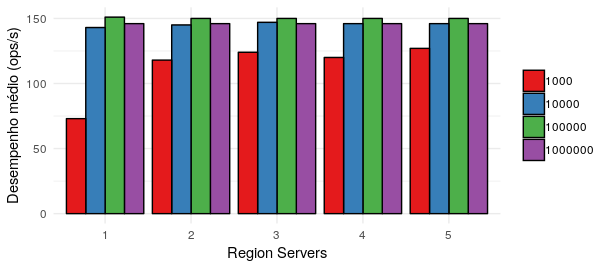
\includegraphics[width=\textwidth]{images/figura21}
        \caption{}
    \end{subfigure}
    \begin{subfigure}[b]{0.49\textwidth}   
        \centering 
        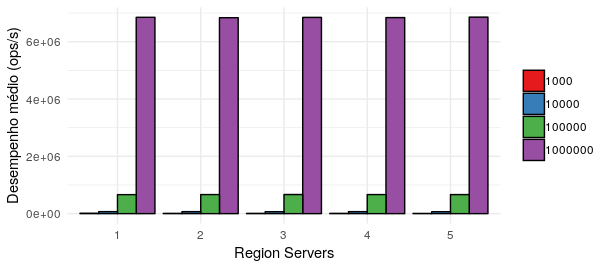
\includegraphics[width=\textwidth]{images/figura22}
        \caption{}
    \end{subfigure}
    \caption{teste}
\end{figure*}

\section{Considerações Finais}
\label{sec:finais}

%\section{Sections and Paragraphs}

%Section titles must be in boldface, 13pt, flush left. There should be an extra 12 pt of space before each title. Section numbering is optional. The first paragraph of each section should not be indented, while the first lines of subsequent paragraphs should be indented by 1.27 cm.

%\begin{figure}[ht]
%\centering
%\includegraphics[width=.5\textwidth]{fig1.jpg}
%\caption{A typical figure}
%\label{fig:exampleFig1}
%\end{figure}

%In tables, try to avoid the use of colored or shaded backgrounds, and avoid thick, doubled, or unnecessary framing lines. When reporting empirical data, do not use more decimal digits than warranted by their precision and reproducibility. Table caption must be placed before the table (see Table 1) and the font used must also be Helvetica, 10 point, boldface, with 6 points of space before and after each caption.

%\begin{table}[ht]
%\centering
%\caption{Variables to be considered on the evaluation of interaction
%  techniques}
%\label{tab:exTable1}
%\includegraphics[width=.7\textwidth]{table.jpg}
%\end{table}


\section{Referências Bibliográficas}

\bibliographystyle{sbc}
\bibliography{sbc-template}

\end{document}
